\documentclass[11pt, english]{report}
\usepackage{graphicx}
\usepackage[colorlinks=true, linkcolor=blue]{hyperref}
\usepackage[english]{babel}
\selectlanguage{english}
\usepackage[utf8]{inputenc}
\usepackage[svgnames]{xcolor}
\usepackage{url}
\usepackage{hyperref}
\usepackage{float}
\usepackage{longtable}
\usepackage[toc]{glossaries}
\usepackage{array}

\usepackage{listings}
\usepackage{afterpage}
\pagestyle{plain}

\definecolor{dkgreen}{rgb}{0,0.6,0}
\definecolor{gray}{rgb}{0.5,0.5,0.5}
\definecolor{mauve}{rgb}{0.58,0,0.82}
\usepackage{biblatex}
\bibliography{ref.bib}

%\lstset{language=R,
%    basicstyle=\small\ttfamily,
%   stringstyle=\color{DarkGreen},
%    otherkeywords={0,1,2,3,4,5,6,7,8,9},
%    morekeywords={TRUE,FALSE},
%    deletekeywords={data,frame,length,as,character},
%    keywordstyle=\color{blue},
%    commentstyle=\color{DarkGreen},
%}

\lstset{frame=tb,
language=R,
aboveskip=3mm,
belowskip=3mm,
showstringspaces=false,
columns=flexible,
numbers=none,
keywordstyle=\color{blue},
numberstyle=\tiny\color{gray},
commentstyle=\color{dkgreen},
stringstyle=\color{mauve},
breaklines=true,
breakatwhitespace=true,
tabsize=3
}

\usepackage{here}


\textheight=21cm
\textwidth=17cm
%\topmargin=-1cm
\oddsidemargin=0cm
\parindent=0mm
\pagestyle{plain}

%%%%%%%%%%%%%%%%%%%%%%%%%%
% La siguiente instrucción pone el curso automáticamente%
%%%%%%%%%%%%%%%%%%%%%%%%%%

\usepackage{color}
\usepackage{ragged2e}

\global\let\date\relax
\newcounter{unomenos}
\setcounter{unomenos}{\number\year}
\addtocounter{unomenos}{-1}
\stepcounter{unomenos}
\gdef\@date{ Course \arabic{unomenos}/ 2019}

\makeglossaries
 


%  kruger
\newglossaryentry{igo}
{
    name=iGo,
    description={The online Ticket Vending Machine Web Application integrating with STM system}
}
\newglossaryentry{traveller}
{
    name=traveller,
    description={People who use STM metros and buses to travel daily in Montreal, Quebec, Canada}
}
\newglossaryentry{stm}
{
    name=STM,
    description={ Société de transport de Montréal (Montreal Transit Corporation)}
}
\newglossaryentry{opus}
{
    name=OPUS,
    description={OPUS is the name of STM travelling card which used by people to travel by STM services, manufactured and distributed by STM agencies}
}
\newglossaryentry{tvm}
{
    name=TVM,
    description={Ticket Vending Machine}
}
\newglossaryentry{cuigo}
{
    name=CUIGO,
    description={Context of use model for iGo}
}
\newglossaryentry{smigo}
{
    name=SMIGO,
    description={Stakeholder  Model representation for iGo}
}
\newglossaryentry{dmigo}
{
    name=DMIGO,
    description={Domain model representation for iGo}
}\newglossaryentry{ucmigo}
{
    name=UCMIGO,
    description={Use Case modelling for iGo}
}



\begin{document}

\begin{titlepage}

\begin{center}
\vspace*{-1in}
\begin{figure}[htb]
\begin{center}

\includegraphics[width=8cm]{images/logo.png}
\end{center}
\end{figure}
\begin{Large}
\textbf{SOEN 6481 - Software System Requirements Specification} \\
\end{Large}
\vspace*{0.1in}
Fall 2019\\
\vspace*{0.5in}
\begin{Large}
\textbf{Requirements Analysis and Elicitation for Ticket Vending Machine} \\
\end{Large}
\vspace*{0.4in}
\begin{large}
Project Report\\
\end{large}
\vspace*{0.2in}
\begin{Large}
\textbf{Deliverable 1} \\
\end{Large}
\vspace*{0.3in}
\begin{large}
Presented to \\
\vspace*{0.1in}
Instructor: PANKAJ KAMTHAN 
 \\
\end{large}
\vspace*{0.3in}
\rule{80mm}{0.1mm}\\
\vspace*{0.1in}
\begin{large}
By \\
\textbf{Team G}\\
Nirav Ashvinkumar Patel - 40081268\\
Rohan Deepak Paspallu - 40093648\\
Jingya Pan - 40044079\\
Divya Pandit - 40087471 \\
Koshaben Patel - 40094385 \\


\end{large}
\vspace*{0.3in}
\textbf{Github URL : https://github.com/niravjdn/SRS-Project}
\end{center}
\end{titlepage}

\newcommand{\CC}{C\nolinebreak\hspace{-.05em}\raisebox{.4ex}{\tiny\bf +}\nolinebreak\hspace{-.10em}\raisebox{.4ex}{\tiny\bf +}}
\def\CC{{C\nolinebreak[4]\hspace{-.05em}\raisebox{.4ex}{\tiny\bf ++}}}

\tableofcontents
\newpage

\chapter{Introduction}
\section{Introduction}
This document is detailed description of \gls{igo}, an electronic ticketing kiosk of public transportation which shall be designed to facilitate individuals of Quebec, Canada.

\section{Purpose}
The purpose of this document is to elicit requirements of stakeholders for problem domain of public transportation. Analysis of requirements is done to provide features to enhance user experience. Stakeholder's requirements is collected by conducting interviews of individuals using \gls{stm}. Furthermore, provision of features is realised by representing problem domain model, context of use model, use case model.

\section{Scope}
This document is applicable for electronic ticket vending machine (iGo) in Quebec, Canada. iGo is an online platform for users allowing them to search fare related queries and perform transcation to recharge \gls{opus}. Scope of development and maintenance part of physical STM ticket vending machine is excluded.   


\chapter{Product Overview}

\section{Problem Statement}
Primary source of public transportation in Montreal, Quebec, Canada is buses and metros. Services of public transport is provided by STM. The current system is designed in such a way that travellers are able to purchase tickets, top up OPUS card using physical ticket vending machines at metro stations. However, OPUS card is not offered by ticket vending machines. Travellers have to recharge OPUS card every month and individuals often stand in queues that causes them inconvenience. Some individuals share the OPUS card to other people and abuse the current system. Prevention of such activity is tiresome for STM officers. There are several reports of lost OPUS card. \\

iGo is proposed to overcome difficulties faced by current system. iGo covers several features of current system and provides solutions to problems faced by individuals.


\section{iGo Description}
iGo is designed to overcome difficulties faced using current system. Solution can be provided by developing web application that \gls{traveller} can use to register, login, recharge OPUS card, manipulate information of profiles. Web application will allow travellers to perform transaction to recharge OPUS card without wasting time in long queues. \\

The traveller is supposed to register into iGo if interaction is happening for the first time. Once they are registered, remaining activities such as finding details of fare, recharging an OPUS card by linking OPUS number to the registered account, scheduling payment can be performed.\\

\begin{figure}[h!]
  
  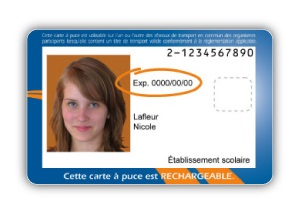
\includegraphics[width=0.5\textwidth]{images/opus-back.jpg}
  \centering
  \caption{Sample image of photo-OPUS card with the unique card number displaying on the back side, provided by STM (Montreal, Quebec, Canada)\cite{card_opus}
}
\end{figure}

iGo is intended to provide following functionalities to facilitate travellers:
\begin{enumerate}
  \item A traveller shall able to register online to iGo system, log into system to manipulate information of profiles.
  \item A traveller shall be able to perform a payment transaction to top-up opus card linked to their account. After login, a traveller will select a top-up amount. The transaction could be made via Debit card, Credit card or Paypal. 
   \item A traveller shall be able to set up scheduled payment for their OPUS card so the amount gets deducted automatically. 
   \item A traveller shall be able to see information related to OPUS card. 
   \item A traveller shall be able to view the OPUS transactions history.
   \item A traveller shall be able to add more than one OPUS cards under one iGo account.
 
   
  \item A traveller shall be able to unlink any OPUS cards under their iGo account.
  
\end{enumerate}

The transaction for payment will be performed by iGo communicating with bank system. iGo will approve the transaction payment once money is deducted from respective bank.\\

The Signup module will stop a traveller if email is used by another user, in this case a traveller must singup using other email address. If a traveller tries to link OPUS that is linked to another iGo account, such activity will be denied by iGo.\\

iGo System will maintain track of its users and their activities such as signup, login, transaction history.

\chapter{Context of Use}
We use the user-centric context of use framework \cite{contextofusecasekamthan}  to identify and classify factors that influence the utility and usability of iGo.\\

\setlength{\tabcolsep}{18pt}
\renewcommand{\arraystretch}{1.5}
\begin{longtable}[!htbp]{ |p{3cm}|p{12cm}| }
\hline
Factor   & Description  \\
\hline

User &  STM Commuters \\
\hline
Experience & 


The commuters who commute on a daily basis using the mode of transportation as Société de transport de Montréal (STM) Bus service as well as the metro service will have their NFC enabled OPUS cards linked to the iGo web application. The interface of the iGo application will have the interface similar to the current system so that the learning curve will not be high and it would be easy for the commuters to accommodate the technology (i.e. understanding the functionality of the OPUS cards, features, etc.). The users who have experience with online purchasing of the goods would find it easy to familiarise themselves with the web app. Moreover, for the users who are not accustomed to online shopping or any online purchase will be provided with a list of guidelines which are needed to be followed to get the benefits of the system.

    \\
\hline
Education &

The commuters who are not familiar with English and French, wont be able to utilise the iGo web application. Moreover, the users who are not accustomed to the computers or mobile won't be able to use the application. So, it's necessary for the commuters to learn the aforementioned things.

 \\
 \hline
Physical Characteristics    &
The users who are visually impaired and who cannot understand the aforementioned languages cannot operate the iGo web service because there is no inbuilt translation and text-reading feature inscribed in the application.
  \\
  \hline
Cognitive Characteristics & 

The people who are familiar with the two languages, as well as have a wide experience of online surfing would get accustomed easily to the iGo app.
  \\
 \hline
Task &  Establishing a connection between the OPUS card and the web application. Moreover, logging in to perform the daily operations.\\
\hline
Complexity &

The Complexity of any application affects the user response as well i.e. if the complexity of the application is high then the there will be a negative customer response. On the contrary, if the application is easier to understand and more user friendly, then it would boost the customer response.
  \\
\hline
Demands &

There is a high demand for the iGo application, because of the following vulnerabilities pertaining in the current system: 
\begin{enumerate}
    \item Long line and burden that explorers must face when they recharge their OPUS cards. \item Visiting the STM ticketing machine for recharging the OPUS card which might not be convenient to many.
    \item Furthermore, STM provides passes as well, so the commuter might not be aware of the number of passes and may run out of passes while in transit.
    \item  Montreal city is one of top 3 cutting edge urban communities in Canada and one of 25 innovative urban communities on the planet. iGo suites the interest of individuals who need to appreciate the comfort of innovation in their STM day by day.\cite{tech_city}
\end{enumerate} \\
\hline 

Workflow Controllability & 

The work process of iGo web application ought to be straightforward for clients to get it. Target end clients could be senior natives or little youngsters who are required to utilize iGo effectively.\\
\hline
Safety & 
As iGo is an online application, authentication and security are the major concepts which were kept in mind while developing the application to incorporate the security features.\\
\hline
Criticality & 
iGo is expected to work precisely. Commuters who pick iGo to top up and deal with their OPUS exchanges can utilize OPUS on all STM metros and bus services. Any blunders caused during on the web exchange procedures are not acknowledged.\\
\hline
Environment & Online and language specific.\\
\hline
Physical Environment & 
So, in order to utilize iGo, voyagers are relied upon to have a PC or cell phone associated with the Internet. Gadgets are relied upon to help web perusing.\\
\hline
\end{longtable}
\vspace*{0.1in}
The above table describes the \gls{cuigo} of iGo\\




%new chapter
\section{Stakeholders}



  Due to the context of use of iGo, a stakeholder mind map has five main branches:
  \begin{enumerate}
      \item iGo Development team 
    \item Quebec Government
    \item Federal Government
    \item STM 
    \item General Public who are travelling via STM transportation in Quebec’s Montreal city. 

\end{enumerate}

iGo development group and STM are two primary partner bunches without whom iGo venture couldn't succeed. Since iGo and STM are identified with an open transportation that works day by day travel benefits in Montreal, Quebec, Canada, two different partners gathering must be broke down, which are the Federal Government of Canada and the Quebec Government. The last partner bunch that straightforwardly uses and appreciates advantages of iGo - Montreal city inhabitants should likewise be dissected.

\section{Stakeholders description}
After discovering stakeholders via mind mapping method, we come up with two main group of stakeholders:
\begin{enumerate}
    \item Non-User stakeholders: Stakeholders who are not end customers of an iGo system. They may be affected by the effect of iGo (unequivocally or oppositely) or they may impact the accomplishment of iGo. We bundle them into Non-User accomplices gathering.
    \item End-User stakeholders:
 The end customers of an iGo system, who genuinely advantage from iGo features and who direct interface with iGo structure.

\end{enumerate}

\subsubsection{Non-user stakeholders}
\vspace*{0.1in}
\setlength{\tabcolsep}{18pt}
\renewcommand{\arraystretch}{1.5}
\begin{longtable}[!htbp]{ |p{3cm}|p{7cm}|p{3cm}| }

\hline
Name & Description & Responsibilities\\
\hline

Quebec Government &
This is a stakeholders who must offer authorizations to let iGo and STM to coordinate. &
Bolster STM and iGo in the law points of view.\\
\hline
Government of Canada and Transport Ministry of Canada  &

This is a stakeholder who must offer authorizations to let iGo and STM incorporate. This partner gathering has a similar power level with Quebec Government in this task. &
Bolster STM and iGo in the law point of view.\\
\hline



STM Office Management &
This is a stakeholder who gives the business rationale and the board support for iGo development group. &
Verify iGo business requirements. 
Advise existing clients about iGo 
Bolster clients during the change from STM TVM to iGo.\\
\hline
iGo Developers & 

This is a stakeholder who must be included routinely to keep up the improvement cycle of iGo.&
Create iGo as per checked business necessities.\\
\hline
iGo Business Analyst &
This is a stakeholder that works with Analysts in STM to accurately make an interpretation of solicitations or necessities into prerequisites to be utilized for advancement. &
Determines subtleties of iGo's functionalities.\\
\hline

iGo Project Manager &
This stakeholder leads the iGo system development. &
Acts as a delegate between the advancement group and the STM. Answerable for following the status of the venture inside spending plan and calendar.\\
\hline
STM Developers &
This is a stakeholder who must be included routinely to keep up the advancement cycle of iGo. &
Develop iGo REST APIs to connect to STM internal system. \\
\hline
STM Business Analyst &
This is a stakeholder that works with analysts in iGo to effectively make an interpretation of solicitations or necessities into prerequisites to be utilized for advancement. &
Indicates subtleties of iGo's functionalities to be good with STM.\\




\hline
STM Project Manager &
This is a stakeholder who is driving for iGo and STM coordination framework advancement. &
Goes about as a middle person between STM specialists and the iGO programming supervisory crew.\\
\hline
Local business who do the top up services for STM card &
  Local organizations have a STM top up charger which enables individuals to top up their OPUS cards without visiting TVM machine in STM workplaces. This partners won't be content with iGo achievement since they will lose their income. \cite{opus_at_home}&


Not applicable\\
\hline

\end{longtable}


\subsection{User stakeholders}
\vspace*{0.1in}
\setlength{\tabcolsep}{18pt}
\renewcommand{\arraystretch}{1.5}
\begin{tabular}{ |p{3cm}|p{4cm}|p{6cm}| }
\hline
Name & Description & Responsibilities\\
\hline

Customers who have STM cards &
Primary users of iGo &
Use iGo online web application for garnish up their OPUS cards and dealing with their STM exchanges. \\

\hline

\end{tabular}

\section{Stakeholders model}
In the wake of examining obligations of partners , we think of the accompanying partner model, portraying their impact to iGo. The further the partners from iGo, the least impact level that they may bring to iGo.


\begin{figure}[H]
  
  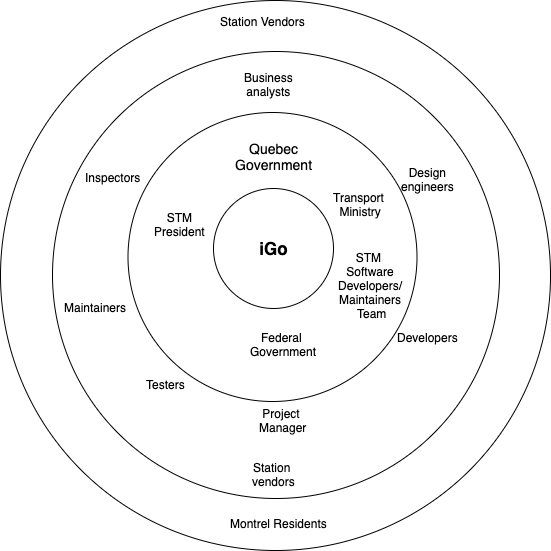
\includegraphics[width=0.8\textwidth]{images/context.png}
  \centering
  \caption{ The Onion model representation for IGO }

\end{figure}
We organize iGo partners dependent on their impact and significance it could be said that without them, iGo will fall flat.
\\
 \begin{itemize}
   \item  Critical
   \begin{itemize}
     \item  The Federal and Quebec Governments has the most noteworthy need since they will give authorizations on iGo's association with STM Cloud just as money for iGo.
    \item The iGO improvement group and STM advancement group has an equivalent impact since they create and keep up iGo framework.\\ \\ \\
   \end{itemize}
   \item  Major
   \begin{itemize}
     \item  The STM agents in the significant rundown as they plan and confirm the necessities of the clients and its representatives.
\item Montreal residents are significant partners since they are immediate clients of the framework. Their inputs and their needs are critical to the accomplishment of iGo.

   \end{itemize}
    \item  Minor
   \begin{itemize}
     \item Neighborhood organizations who administration clients to top up OPUS cards through their OPUS scanners are the least impact partners. They have no duties and less to state about iGO.

   \end{itemize}
 \end{itemize}
 
  \begin{figure}[H]
  
  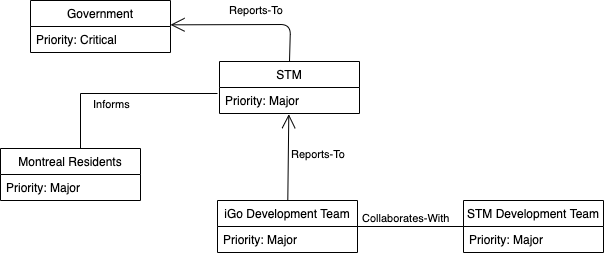
\includegraphics[width=0.8\textwidth]{images/stake_relationship.png}
  \centering
  \caption{ Stakeholders relationship model}

\end{figure}



\chapter{Domain Model}
\section{Problem Domain Model}

% domain model description
Followings are the concepts that are depicted in the domain model:\\
\begin{itemize}
  \item STMUser: A generic term of the user who interact with the IGo system, for the IGo system, the potential user including regular citizen, student, senior citizen, children and differently abled user.
  \item OPUSCard: The physical artifact that helps the user to interact with the system.
  \item IGoAccount: For the sake of the using the system more convenient, a specific IGo account is created for each user.
  \item Transaction: A composition of the functionalities included in the system, the user are able to initialize the transaction,including register the account, inquiry the balance, deposit the money, and obtain invoice.
  \item Payment: Certain transaction will need the user to pay. For example, deposit in the account.
\end{itemize}
\bigskip
From the domain model of the IGo system, we can clearly see the properties of each concepts listed above and the relationships between these concepts.
\begin{itemize}
\item Between the IGoAccount and the STMUser, a one-to-one relationship is exist. For the IGo system, each user in the system will be given a unique account to interact with the system.
\item Between the STMUser and the Transaction,a one-to-many relationship is exist. For the IGo system, a user are able to initialize multiple transaction, however for each specific transaction, only one user will be involved.
\item Between the Transcation and the payment, a ont-to-one relationship is exist. For a specific transaction, a unique payment operation will be initialized. And for a specific payment operation,exist a specific transaction only.
\item There is a generalize relationship between STMUser and several specific user type, as mentioned above, regular citizen, student, senior citizen, children and differently abled user.

\item There is a generalize relationship between  Transaction and several specific transcation type, as mentioned above,  register the account, inquiry the balance, deposit the money, and obtain invoice.

\end{itemize}

 \begin{figure}[H]
  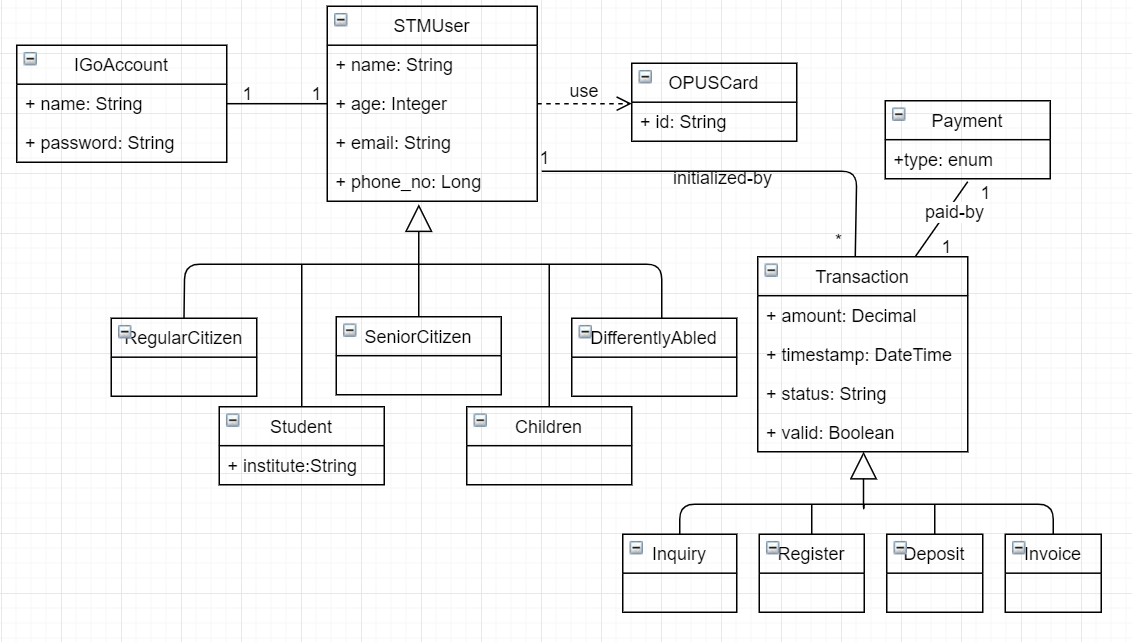
\includegraphics[width=1.0\textwidth]{images/domainModelSTM.png}
  \centering
  \caption{Domain Model of IGo (\gls{dmigo})}
\end{figure}


\chapter{Use Case Model }
\section{Use Case Diagram}
 \begin{figure}[H]
  
  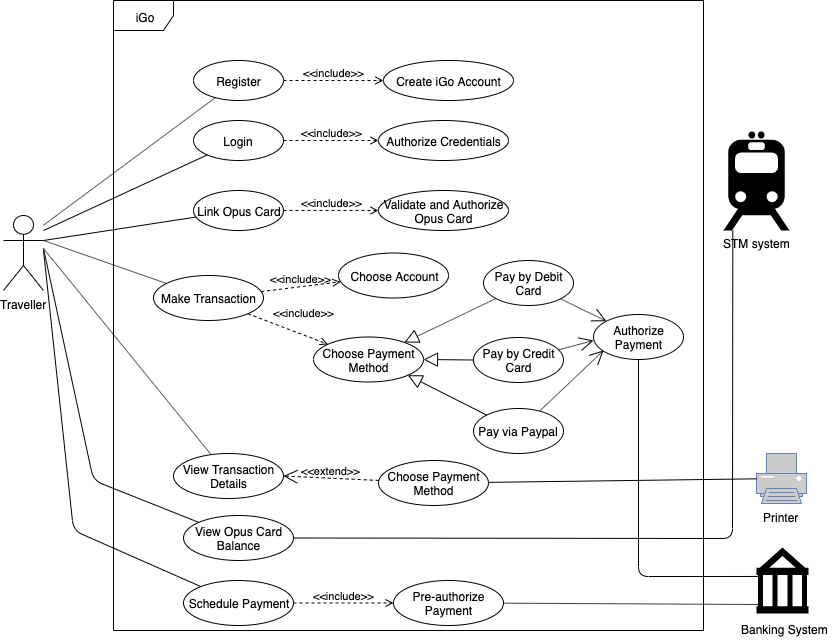
\includegraphics[width=0.8\textwidth]{images/usecase.png}
  \centering
  \caption{Use case model of iGo (\gls{ucmigo})}

\end{figure}

\begin{figure}[H]
  
  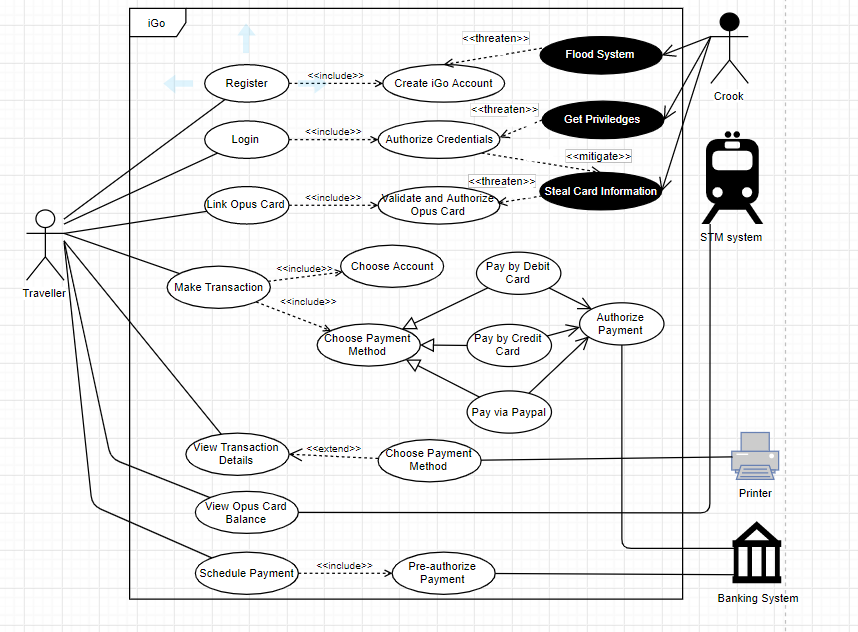
\includegraphics[width=0.8\textwidth]{images/negativeusecase.png}
  \centering
  \caption{ Negative Use case model of iGo (\gls{ucmigo})}

\end{figure}

 \begin{figure}[H]
  
  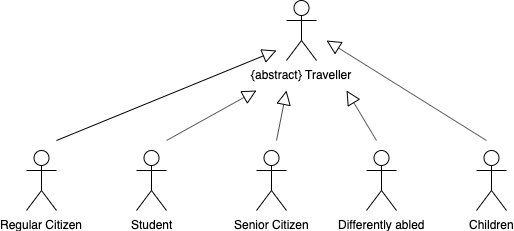
\includegraphics[width=0.8\textwidth]{images/actor_relationship.png}
  \centering
  \caption{Types of Actors and relationship between them in iGo}

\end{figure}



\section{Use Case Brief}

Register an account in iGo System and carry out successful payment for OPUS card\\
Actor: STM customers/Travellers\\

\textbf{Login} : A STM customer needs to register to iGo system using his/her email address. iGo will authenticate a user with STM system via Remote APIs developed by STM developers. iGo will display error or successful message based on the response returned by the STM to the customer.The Customer must wait to receive a notification from STM inorder to make a payment for the OPUS Recharge.\\ 

\textbf{Link OPUS Card} : After successful Login the iGo system will Link the customers account to the internal STM system wherein further validation will take place and response will be sent by the STM system to customer to choose and enter appropriate payment details for successful payment/recharge of OPUS card.\\ 

\textbf{Make Transaction }: 
Once the payment details are entered by the customer the iGo will connect to the respective banking system of customer to validate entered card details.Before entering the payment details the customer needs to be careful about the details he/she is entering as the details if leaked can lead to negative effects.\\  

\textbf{Schedule payment} : 
If the card is validated successfully the payment is done and the opus Card user gets a receipt of successful payment,else the banking system notifies the iGo  that card details entered are not valid.The iGo then requests customer to make new account and carry out payment process.\\ 

\textbf{View Transaction details} : 
Once a transaction is complete the customer gets the receipt for the successful payment for OPUS card which includes the details of transaction that customer can verify. \\

\subsubsection{Fully Dressed Use-Case Scenario - Success scenario}
\vspace*{0.1in}
\setlength{\tabcolsep}{18pt}
\renewcommand{\arraystretch}{1.5}
\begin{tabular}{ |p{4cm}|p{10cm}|}
\hline
Use case Section & Comment\\
\hline

Use case Name & Successful Reload of OPUS at ticket vending machine of STM\\
\hline

Scope &
 iGo plays as an online platform allowing travellers to load  their  OPUS  cards  and  manage  STM  transactions  themselves for successful everyday travel with ease with convenience. \\
\hline
Primary Actor & Daily Traveller's/STM users \\
\hline
StakeHolders & iGo Developers/STM Developers/Government of Canada and Transport Ministry of Canada/Quebec Government \\
\hline

\end{tabular}


\setlength{\tabcolsep}{18pt}
\renewcommand{\arraystretch}{1.5}
\begin{tabular}{ |p{4cm}|p{10cm}|}
\hline
Pre-Condition & Customer will try to log in the system with his private credentials. \\
\hline
Post-Conditions & customer successfully reloads the OPUS card for travel and gets the receipt of the transaction from the iGo system.\\
\hline
Main Scenario & Steps:
\begin{enumerate}
  \item Customer will try to log in the system with his private credentials.
  \item After successful login the system will prompt the customer to choose Opus recharge option.
  \item Customer will select the Opus recharge option.
  \item Customer will choose Payment options.
  \item Customer will enter payment details.
  \item Card will be validated by the system internally by connecting to correspondent banking system.
  \item  Card is validated successfully by the bank.
  \item Opus card is successfully recharged
  \item customer successfully reloads the OPUS card for travel and gets the receipt of the transaction from the iGo system.
  
\end{enumerate}

\\
\hline
Extensions &
\begin{enumerate}
  \item During payment customer can choose between cash or digital payment.
  \item customer can select for in paper receipt or email notification of the successful recharge.
  
\end{enumerate}


Not applicable\\
\hline
Frequency of occurrence &
monthly or biweekly(rarely)\\

\hline
Open Issues & customer needs and payment details details or could result in negative consequences.\\
\hline
\end{tabular}



%sequence diagram goes here

\begin{figure}[H]
  
  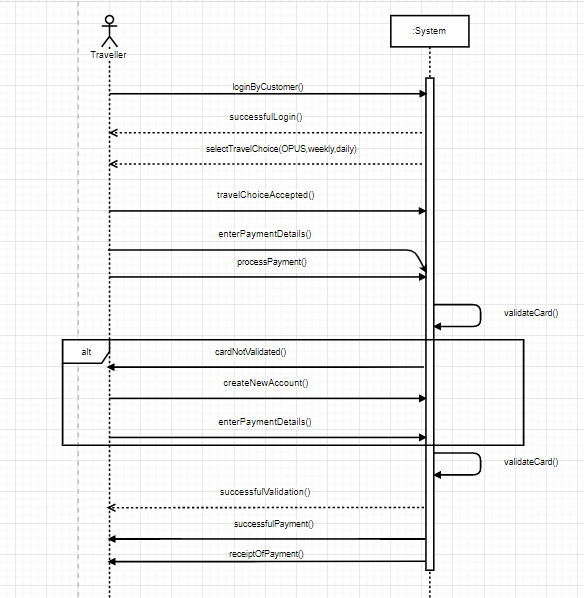
\includegraphics[width=0.8\textwidth]{images/ssd.png}
  \centering
   \caption{Sequence Diagram for TVM}

\end{figure}

% System sequence diagram goes here
\begin{figure}[H]
  
  \includegraphics[width=0.8\textwidth]{images/SSD.PNG}
  \centering

   \caption{Sequence Diagram for TVM}

\end{figure}


% Activity diagram goes here
\begin{figure}[H]
  
  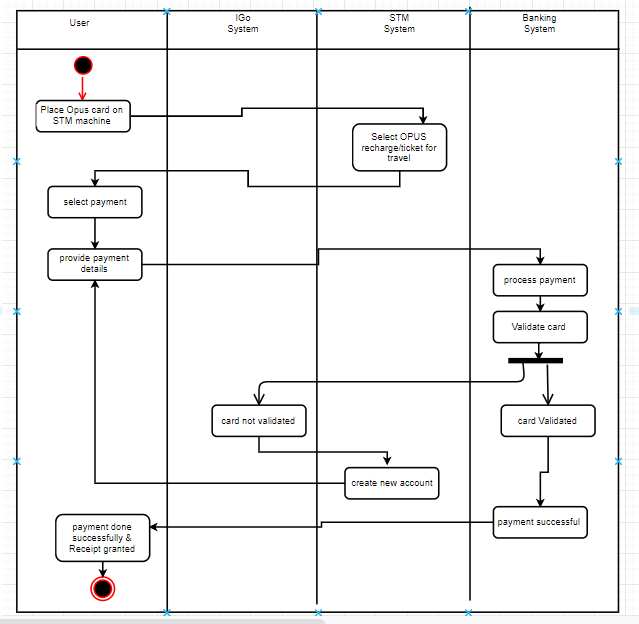
\includegraphics[width=0.8\textwidth]{images/Activity.PNG}
  \centering

   \caption{Activity Diagram for payment case}

\end{figure}




\appendix
\chapter{Interview}
Interviews\cite{interview} were conducted with two primary users, an international student and a teaching assistant. Interviews are done to gain more understanding about the system in order to build the correct requirements. The answers to the questions are written in both active and passive voice for the user to have a better understanding. We have done one pilot interview(with TA) and four regular interviews. For the interviews done, we have implemented the funnel technique of interviewing in which we begin from general questions and move to specific questions.


\section{Pilot Interview}
\textbf{Date-} 09-23-2019\\
\textbf{Time-} 8:45 PM to 9:00 PM\\
\textbf{Interviewers:}\\

\textbf{Name:} ROHAN DEEPAK PASPALLU \\
\textbf{Institute:} Concordia University, Montreal \\
\textbf{Industry:} Educational sector\\
\textbf{Title:} Student \\ 

\textbf{Interviewee:}\\

\textbf{Name:} Samia Hilal \\
\textbf{Institute:} Concordia University, Montreal \\
\textbf{Industry:} Educational sector\\
\textbf{Job Title:} Teaching Assistant\\ 


\textbf{Generic Questions:}\\

Question: What do you study at Concordia University? \\
Answer: I am not a student, I am a Teaching Assistant for the subject Software Requirements Specification.

\textbf{Transportation Used:}\\

Question: How often do you use STM transportation and why you do you prefer STM over other transportation methods?\\
Answer: Here in Montreal, the major mode of transportation is the STM. Moreover, I am not the best person to ask the question because honestly speaking I drive my own car. But, I think STM is good and I like using it when I can. At the moment, I use STM twice a month.\\

Question: How easy is it to access STM services from your residence?\\
Answer: Actually, its not bad, its quite easy. It takes me 90 minutes to reach the university. Its easy to access the STM, but the travel duration is long.\\

\textbf{Gadgets Used:}\\

Question:What gadgets you use on a daily basis?\\
Answer: I use my mobile phone while travelling.\\

Question: How often you access these devices?\\
Answer: I use it to access the schedule of the bus and the map service.\\

Question: Which do you prefer using the most?\\
Answer: I prefer driving my own card..\\

Question: Are you comfortable using these devices?\\
Answer: Yes, its been a part of our lives now a days.\\

\textbf{Family Specifics:}\\

Question: Are there any dependents or young members in your family and how many?\\
Answer: No, there is no one dependent on me. \\

\textbf{Specific Questions:}\\

Question: When do you purchase tickets for your travel?\\
Answer: I usually take an OPUS card and load 10 tickets into it because I am not a frequent user, I am an occasional user. When there are any events in the downtown and I have to come a lot in the weekend, then I prefer buying the weekend passes.\\

Question: What are the difficulties you face when purchasing a ticket?\\
Answer: I have to go to the pharmacy to recharge my OPUS card, so I wish there was something through which I can recharge my OPUS without going anywhere and buy the tickets from your own home.\\

Question: Do you have any worst experiences with the STM?\\
Answer: No, its generally okay.\\

Question: Will you prefer a system that enables you to recharge anytime and anywhere?\\
Answer: Of course, that would be perfect, because i have kids and I have to buy tickets for them and we have to rush for the tickets in the morning or any time of the day, so its better if we could recharge the OPUS from the home. \\

Question: Do you encounter the first day of the month problem wherein it is mandatory to load the
card even though you have used it only for 15 days?\\
Answer: Sorry, I am not the right person to ask this question as I am not a frequent user.

Questions: Do you face any problems while performing any transaction ?
Answer: No, its actually fun.

Question: What would love to see changed?\\
Answer: As I mentioned before, that the online reloading the OPUS card would be a great relief for all. I would like to have a digital card, as I have a daughter and she frequently looses her OPUS card.\\

Question: Assume you are using an online application to buy your tickets. To register into the system, do you prefer providing your phone number, email , both / neither? Why?\\
Answer: Yes, I'm okay with providing both information.\\
 

 
Question: Do you  need an option to save your application logged-in in the device so next time the user doesn’t need to login again?\\
Answer: Yes, I would prefer stay logged-in.\\

Question: Would you wish to receive an email or message in advance for scheduling your recharge for OPUS card?\\
Answer: Yes, I would love that because there are many things to remember and we tend to forget things.\\
 
 
Question: If yes, how many days in advance that a user wants to receive an informing email?\\
Answer: yes, one week would be good according to me.\\

Question: Do you think that the concept of digitization would be understood and accepted by all age groups ?\\
Answer: Its a choice, but I see many elderly people using these things. Almost everyone uses virtual cards and so on.\\

Question:Do you think that the change would create any havoc or problems for the people ?\\
Answer: I think there should be some security measures for verifying the picture or any such thing for the reduced rate or any such thing.\\

Question: Do you have some suggestions which could be incorporated by the STM ?\\
Answer: I think they need to be more efficient and reduce long queues and waiting times. Moreover, the interface is very bad, so the user interface should be better.\\
Thank you so much for your time. Mrs. Samia Hilal! It was a pleasure speaking with you. \\





\section{Interview 1}
\textbf{Date-} 09-27-2019\\
\textbf{Time-} 11:15 AM to 11:45 AM\\
\textbf{Interviewers:}\\

\textbf{Name:} Nirav Patel \\
\textbf{Institute:} Concordia University, Montreal \\
\textbf{Industry:} Educational sector\\
\textbf{Title:} Students \\ 

\textbf{Interviewee:}\\

\textbf{Name:} Darshan Patel \\
\textbf{Institute:} Concordia University, Montreal \\
\textbf{Industry:} Educational sector\\
\textbf{Job Title:} Graduate Student\\ 


\textbf{Generic Questions:}\\

Question: What do you study at Concordia University? \\
Answer: I study Master's of Mechanical Engineering at Concordia University.

\textbf{Transportation Used:}\\

Question: How often do you use STM transportation and why you do you prefer STM over other transportation methods?\\
Answer: I use metro on a daily basis. It helps me commute to university and work many times. I also take bus on weekends if I’m about to sightsee or walk in Walmart or Costco.\\

Question: How easy is it to access STM services from your residence?\\
Answer: It's easy to access it from my home. It's only 2 min away from home.\\

\textbf{Gadgets Used:}\\

Question:What gadgets you use on a daily basis?\\
Answer: I use my mobile phone while travelling.\\

Question: How often you access these devices?\\
Answer: I use almost for an entire journey actively or listening songs.\\

Question: Which do you prefer using the most?\\
Answer: I prefer using metro.\\

Question: Are you comfortable using these devices?\\
Answer: Ye, because I use them on daily basis.\\

\textbf{Family Specifics:}\\

Question: Are there any dependents or young members in your family and how many?\\
Answer: No, there is no one dependent on me. \\

\textbf{Specific Questions:}\\

Question: When do you purchase tickets for your travel?\\
Answer: I reload my card every month.\\

Question: What are the difficulties you face when purchasing a ticket?\\
Answer: Sometimes, it's very difficult, I will have to wait in a long queue to reload my card..\\

Question: Does it irritate standing in long queues?\\
Answer: Yes, when I'm in rush it takes a lot time.\\

Question: Will you prefer a system that enables you to recharge anytime and anywhere?\\
Answer: Of course, I would love that. It would be easy and fast. \\

Question: Do you encounter the first day of the month problem wherein it is mandatory to load the
card even though you have used it only for 15 days?\\
Answer: Yes, it is difficult.\\

Question: Have you used any web application for your transactions previously? If yes, which one? \\
Answer: Yes, I have used applications like Tim Hortons.\\

Question: What did you like about the application?\\
Answer: The application are good and easy to use. It saves time also.\\

Question: Was it easy to use?\\
Answer: Yes, very easy.\\

Question: Any difficulties you faced when performing a transaction?\\
Answer: No, actually not.\\

Question: What would love to see changed?\\
Answer: The application we use, should be very secure. Security should be prioritized.\\

Question: Assume you are using an online application to buy your tickets. To register into the system, do you prefer providing your phone number, email , both / neither? Why?\\
Answer: No preference, I'm okay with providing both information.\\
 
Question: Once you register, do you prefer the account verification to activate your account to redirect to email/phone to make it more secure?\\
Answer: Yes I would. If it’s more secure then I would do it.\\
 
Question: Do you want to receive a confirmation message via their registered phone/Email?\\
Answer: Yes, I would like to have that.\\
 
Question: Do you  need an option to save your application logged-in in the device so next time the user doesn’t need to login again?\\
Answer: Yes, I would prefer stay logged-in.\\

Question: Which are the online payments that you use?\\
Answer: I would prefer paypal, as it's more secure and does not require credit card information on end site.\\
 
Question: What is your predominant mode of transaction?\\
Answer: Just Tap and Pay.\\
 
Question: Do you want to save their payment credentials to save time during your upcoming transactions?\\
Answer: Yes\\
 
Question: Do you wish to receive in advance email informing that your schedule payment will be in, let’s say, next 2 days?\\
Answer: Yes, that would be helpful, that would help me keeping track of my transactions.\\
 
Question: If yes, how many days in advance that a user wants to receive an informing email?\\
Answer: yes, 5 days would be good according to me.\\

Thank you so much for your time. Mr. Darshan! It was a pleasure speaking with you. \\


\newpage
\section{Interview 2}
\textbf{Date-} 10-03-2019\\
\textbf{Time-} 15:30 PM to 15:45 PM\\
\textbf{Interviewers:}\\

\textbf{Name:} Jingya Pan \\
\textbf{Institute:} Concordia University, Montreal \\
\textbf{Industry:} Educational sector\\
\textbf{Title:} Students \\ 

\textbf{Interviewee:}\\

\textbf{Name:} Bingyu An \\
\textbf{Institute:} Concordia University, Montreal \\
\textbf{Industry:} Educational sector in Finance Falcuty\\
\textbf{Job Title:} Graduate Student\\ 


\textbf{Generic Questions:}\\
Question: How many times you use the STM system per
week in Montreal? \\\\
Answer: I use it almost everyday. Because i do not live in Dt, therefore i need to take the metro to get to school. Except the day i have class, i also go to the library to review the lessons. During the weekend, i will go to the old port to have a walk or go to the supermarket, so i am really a regular customer for STM.\\

Question: For the STM system, what is feature that you like most?\\\\
Answer: I think the STM system is considerable which provides several type of ticket to satisfy the people's needs. For me, I get a student card, so I can get a student discount with fixed amount of money and take the metro and bus unlimited times. As I know, the metro also provides a specific ticket type after 5pm which is less expensive than the normal ticket type.\\


Question: What is the main problem of the STM system from your perspective?\\\\
Answer: That should be renew the OPUS card especially on the weekend. I still remembered once that happened. It was a Saturday, so there was no cashier service, the only way to renew the card is to do it through the machine in the metro station, it was so many people in line, which took me a long time to wait.\\

Question: If the STM system provides an extra service for the online charging, do you think it will be helpful?\\\\
Answer: I think it would be much better, as the majority people are able to be accessible to the internet and most of the people are familiar with the online service, so at least half of the people probably will use the online service and rest can still go to the cashier or use the machine in the metro station. At least, it will not be that crowded.\\



\section{Interview 3}
\textbf{Date-} 09-29-2019\\
\textbf{Time-} 15:15 PM to 15:45 PM\\
\textbf{Interviewers:}\\

\textbf{Name:} Divya Pandit \\
\textbf{Institute:} Concordia University, Montreal \\
\textbf{Industry:} Educational sector\\
\textbf{Title:} Students \\ 

\textbf{Interviewee:}\\

\textbf{Name:} Aditya Surve \\
\textbf{Institute:} Concordia University, Montreal \\
\textbf{Industry:} Educational sector\\
\textbf{Job Title:} Graduate Student\\ 


\textbf{Generic Questions:}\\

Question: What do you study at Concordia University? \\
Answer: I study Master's of Software Engineering at Concordia University.

\textbf{Transportation Used:}\\

Question: How often do you use STM transportation and why you do you prefer STM over other transportation methods?\\
Answer: I use metro on a daily basis. It helps me commute to university and work many times. I also use STM buses mostly as it helps me reach places quicker and smoothly where metro might take some longer time.Its convienient some time like going to walmart or shopping places that are mostly located away from metro stations.\\

Question: How easy is it to access STM services from your residence?\\
Answer: It's easy to access it from my home as I have a bus stop just below my building.\\

\textbf{Gadgets Used:}\\

Question:What gadgets you use on a daily basis?\\
Answer: I use my mobile phone while travelling.\\

Question: How often you access these devices?\\
Answer: I use my phone almost for an entire journey actively, listening songs,watching youtube videos sometimes.\\

Question: Which do you prefer using the most the metro or the bus?\\
Answer: I prefer using metro as well as both. I like both of them.\\

\textbf{Family Specifics:}\\

Question: Are there any dependents or young members in your family and how many?\\
Answer: No, there is no one dependent on me.All live in my home country.I live here with my friends. \\

\textbf{Specific Questions:}\\

Question: When do you purchase tickets for your travel?\\
Answer: I reload my card every month.Its anyways hectic to recharge on the first day of the month as the stations have long queues to recharge opus card on the first day of the month.\\

Question: What are the difficulties you face when purchasing a ticket?\\
Answer: Sometimes, it's very difficult,I mentioned on the first day its too much rush on station.\\

Question: Does it irritate standing in long queues?\\
Answer: Yes, when I'm in rush it takes a lot time of my precious time.I am in a hurry to reach somewhere.yes its damn irritating\\

Question: Will you prefer a system that enables you to recharge anytime and anywhere?\\
Answer: Of course, I would love that. It would be easy and fast. \\

Question: Do you encounter the first day of the month problem wherein it is mandatory to load the
card even though you have used it only for 15 days?\\
Answer: Yes, it is difficult.

Question: Have you used any web application for your transactions previously? If yes, which one? \\
Answer: Yes, I have used applications like Tim Hortons,amazon,starbucks etc.

Question: What did you like about the application?\\
Answer: The application are good,portable and easy to use. It saves lot of time also.\\

Question: Was it easy to use?\\
Answer: Yes, very easy.\\

Question: Any difficulties you faced when performing a transaction?\\
Answer: No, actually not.Sometimes its due to internet issues but that is still fine.\\

Question: What would love to see changed?\\
Answer: The application we use, should be more privatized and portability importantly should be prioritized.\\

Question: Assume you are using an online application to buy your tickets. To register into the system, do you prefer providing your phone number, email , both / neither? Why?\\
Answer: No problem im okay with that but it needs to be taken care of.The information should remain confidential.\\
 
Question: Once you register, do you prefer the account verification to activate your account to redirect to email/phone to make it more secure?\\
Answer: Yes I would. If it’s more secure then I would do it.\\
 
Question: Do you  need an option to save your application logged-in in the device so next time the user doesn’t need to login again?\\
Answer: Yes, I would prefer stay logged-in.\\

Question: Which are the online payments that you use?\\
Answer: I would prefer paytm,transferwise as its more secure and easy to go with family and friends.\\
 
Question: What is your predominant mode of transaction?\\
Answer: Digital anytime.\\
 
Question: Do you want to save their payment credentials to save time during your upcoming transactions?\\
Answer: No\\
 
Question: Do you wish to receive in advance email informing that their schedule payment will be in, let’s say, next 2 days?\\
Answer: Yes, that would be helpful, that would help me keeping track of my transactions.\\

Thank you so much for your time. Mr.Aditya! It was a pleasure speaking with you. \\


\section{Interview 4}
\textbf{Date-} 09-30-2019\\
\textbf{Time-} 15:15 PM to 15:35 PM\\
\textbf{Interviewers:}\\

\textbf{Name:} Koshaben Patel \\
\textbf{Institute:} Concordia University, Montreal \\
\textbf{Industry:} Educational sector\\
\textbf{Title:} Students \\ 

\textbf{Interviewee:}\\

\textbf{Name:} Deep Patel \\
\textbf{Institute:} Concordia University, Montreal \\
\textbf{Industry:} Educational sector\\
\textbf{Job Title:} Undergraduate Teaching Assistant\\ 


\textbf{Generic Questions:}\\

Question: What do you study at Concordia University? \\
Answer: I study master's in applied computer science at Concordia University.

\textbf{Transportation Used:}\\

Question: How often do you use STM transportation and why you do you prefer STM over other transportation methods?\\
Answer: I use services of STM transportation frequently. I don't own a car, I rely on the services of STM. I use STM transportation over other mode of transport because of the convenience and fits my budget also.\\

Question: How easy is it to access STM services from your residence?\\
Answer: It's easy to access STM services as I live in downtown. My home is one block away from guy concordia metro station, so it's really easy to access services of STM.\\

\textbf{Gadgets Used:}\\

Question:What gadgets you use on a daily basis?\\
Answer: On daily basis, mobile phone and laptop is used. Usage of laptop is comparatively higher than mobile phone.\\

Question: How often you access these devices?\\
Answer: I heavily use laptop and mobile phone. I use it for different purposes and that ranges from study, work, entertainment. \\

Question: Which do you prefer using the most the metro or the bus?\\
Answer: There is no such preference. However, I like metro more because in winter it's freezing to death.\\

\textbf{Family Specifics:}\\

Question: Are there any dependents or young members in your family and how many?\\
Answer: No, nobody is dependent on me. It is best I think. \\

\textbf{Specific Questions:}\\

Question: When do you purchase tickets for your travel?\\
Answer: I don't purchase tickets. As I am student, I reload OPUS every month. Most of the time, because of my busy schedule I end up reloading opus in the beginning of the month.\\

Question: What are the difficulties you face when purchasing a ticket?\\
Answer: One of the obvious difficulties is to stand in long queue to reload opus card, it is tiresome activity to be honest. It gets even more annoying because I am always rushing and sometimes people ahead me take forever to buy the tickets, I don't know what is the matter with them. Maybe some of them are tourists I assume. But yes, standing in queue is the difficulty I face when reloading opus card. \\

Question: Does it irritate standing in long queues?\\
Answer: Yes, as I said, it is tiresome activity and I hate to wait.\\

Question: Will you prefer a system that enables you to recharge anytime and anywhere?\\
Answer: Definitely. It will be a heaven on earth. I think many people will be happy to have the kind of system that lets them buy or recharge their cards. \\

Question: Have you used any web application for your transactions previously? If yes, which one? \\
Answer: Yes, I have used web applications such as amazon, flipkart, domino's pizza, fido and many more.

Question: What did you like about the application?\\
Answer: Those applications are convenient and the amount of time saved is something I love a lot. It almost eliminates need for cash currency for payment and I love it.\\

Question: Was it easy to use?\\
Answer: Yes, those applications are designed in such a way that most people are comfortable especially people of my generation. I can't say whether oldies find it easy to use.\\

Question: Any difficulties you faced when performing a transaction?\\
Answer: I don't remember me facing any troubles. It was great experience performing transactions online.\\

Question: What would you love to see changed?\\
Answer: I am concerned with security, I won't like if my private information is leaked. So, I will want those applications to provide me security. One more thing, I will be happy if STM provides some sort of discounts for regular customers or they should come up with subscription plans. \\

Question: Assume you are using an online application to buy your tickets. To register into the system, do you prefer providing your phone number, email , both / neither? Why?\\
Answer: Yes, I am comfortable with me sharing information as long as privacy is not compromised. However, It takes me time to trust on organisations. I hear others' experience and then I am comfortable sharing the information.\\
 
Question: Once you register, do you prefer the account verification to activate your account to redirect to email/phone to make it more secure?\\
Answer: Yes. It is a secured way to perform transaction activity. I prefer that step to be taken by any organisation.\\
 
Question: Do you need an option to save your application logged-in in the device so next time the user does not need to login again?\\
Answer: Yes, to log into system I wouldn't want to enter password every time as most of the time I log into system using my private computer. \\

Question: Which are the online payments that you use?\\
Answer: I use PayPal, and bunch of banking applications for purchasing stuff.\\
 
Question: What is your predominant mode of transaction?\\
Answer: I use credit card most of the time. I send money to my friends using interac feature of scotia bank. All the transactions are done using mobile banking application.\\
 
Question: Do you want to save their payment credentials to save time during your upcoming transactions?\\
Answer: Yes. As I said before, I wouldn't want to enter my details manually all the time.\\
 
Question: Do you wish to receive in advance email informing that their schedule payment will be in, let’s say, next 2 days?\\
Answer: Yes, It will be helpful if I am sent an email regarding schedule payment.\\

Thank you so much Mr.Deep. Given information is valuable to me. Thanks for participation. \\


\newpage
\chapter{Team Contribution}

\begin{center}
\begin{tabular}{ | m{20em} | m{8cm}| } 
\hline
 Problem 1: Brief description& Nirav Patel,Rohan Deepak Paspallu,Jingya Pan,
Divya Pandit,Koshaben Patel\\ 
\hline
Problem 2: Context of use model & Nirav Patel,Rohan Deepak Paspallu,Jingya Pan,
Divya Pandit,Koshaben Patel\\ 
\hline
Problem 3: Problem domain model & Nirav Patel,Rohan Deepak Paspallu,Jingya Pan,
Divya Pandit,Koshaben Patel\\ 
\hline
Problem 4: Use case model & Nirav Patel,Rohan Deepak Paspallu,Jingya Pan,
Divya Pandit,Koshaben Patel\\ 
\hline
Interview & Nirav Patel,Rohan Deepak Paspallu,Jingya Pan,
Divya Pandit,Koshaben Patel\\ 
\hline
\end{tabular}
\end{center}


\newpage
\printbibliography
\newpage
\printglossary

\end{document}